\documentclass[8pt,twoside]{scrartcl}

% Pakete einbinden
\usepackage[utf8]{inputenc}
\usepackage[ngerman]{babel}
\usepackage[babel]{csquotes}
\usepackage{sourcesanspro}
\usepackage{sourcecodepro}
\usepackage[default,regular,black]{sourceserifpro}
\usepackage[official]{eurosym}
\usepackage[a6paper,inner=1.25cm,outer=1cm,bottom=1cm]{geometry}
\usepackage{textpos}
\usepackage{longtable}
\usepackage{tabu}
\usepackage{booktabs}
\usepackage{hyperref}
\usepackage[hyphenbreaks]{breakurl}
\usepackage{graphicx}
% Wo liegen die Bilder
\graphicspath{{./images/}}
\usepackage{rotating}
\usepackage{setspace}
\onehalfspacing
\renewcommand{\arraystretch}{1.5}
\setlength{\parindent}{0pt}
\usepackage{enumitem}
\usepackage{calc}
\usepackage{ifthen}
\usepackage{intcalc}

\setcounter{secnumdepth}{0} % Überschriften nicht nummerieren.
\newcommand{\email}[1]{{\UrlFont\href{mailto:#1}{#1}}}

\title{Ersti-Hilfe für die Institute für 
    Mathematik und Informatik zum
    Wintersemester 2018/19}
\author{Fachschaftsrat Mathematik/Informatik}
\date{\today}

\usepackage{scrlayer-scrpage}
\ofoot{}
\ohead*{\sffamily\thepage}
\ihead{\sffamily\leftmark}

\usepackage{datatool}
\newcommand{\definition}[2]{\DTLnewrow{list}\DTLnewdbentry{list}{key}{#1}\DTLnewdbentry{list}{description}{#2}}
\newenvironment{encyclopedia}{%
    \DTLifdbexists{list}{%
        \DTLcleardb{list}%
    }{%
        \DTLnewdb{list}%
    }%
}{%
    \DTLsort*{key}{list}%
    \begin{description}[itemsep=0.5ex]%
        \DTLforeach*{list}{%
            \theKey=key, \theDesc=description%
        }{
            \item[\theKey] \theDesc
        }%
    \end{description}%
}

\usepackage{relsize}
\renewcommand{\UrlFont}{\sffamily\smaller}
% \makeatletter
% % Inspired by http://anti.teamidiot.de/nei/2009/09/latex_url_slash_spacingkerning/
% % but slightly less kern and shorter underscore
% \let\UrlSpecialsOld\UrlSpecials
% \def\UrlSpecials{\UrlSpecialsOld\do\/{\Url@slash}\do\_{\Url@underscore}}%
% \def\Url@slash{\@ifnextchar/{\kern-.11em\mathchar47\kern-.2em}%
%     {\kern-.0em\mathchar47\kern-.08em\penalty\UrlBigBreakPenalty}}
% \def\Url@underscore{\nfss@text{\leavevmode \kern.06em\vbox{\hrule\@width.3em}}}
% \makeatother

\usepackage{xcolor}
\definecolor{coverbackground}{RGB}{255,138,228}
\definecolor{coverforeground}{RGB}{72,22,54}

\begin{document}

% Titelseite
\thispagestyle{empty}
\pagecolor{coverbackground}
\color{coverforeground}
\newgeometry{margin=1cm,inner=1.25cm}
{
    \setlength{\parindent}{0pt}
    \sffamily
    \begin{textblock*}{\textwidth}(0cm, 0cm)%
        \hspace*{\stretch{1}}
        \begin{sideways}
            \begin{minipage}{\textheight}
                \fontsize{1.5cm}{1.5cm}\selectfont%
                \bfseries
                \hspace{-0.1em}
                Ersti-Lexikon ’20
                \hfill
            \end{minipage}
        \end{sideways}%
    \end{textblock*}
    {
        \fontsize{0.45cm}{0.45cm}\selectfont
        Martin-Luther-Universität \hfill
        Halle-Wittenberg
    }
    \vfill
    
\includegraphics[width=0.6\linewidth]{turtle} \\[0.5cm]
    {%
        \fontsize{0.675cm}{0.675cm}\selectfont
        Fachschaftsrat \\[0.5ex]
        Mathematik/Informatik
    }%
}%
\newpage
\restoregeometry
\nopagecolor
\color{black}

% Impressum
\thispagestyle{empty}
\vspace*{\stretch{1}}
\subsubsection{Impressum}
\begin{tabu} to \textwidth {@{}lX@{}}
    Herausgeber: & Fachschaftsrat Mathematik/Informatik der
        Studierendenschaft der Martin-Luther-Universität Halle-Wittenberg K.d.ö.R. \\
    Autoren: &
        Peter Böttcher,
        Jan Heinrich Reimer,
        Aaron Gröbel,
        Anna Hemmann,
        Tuğçe Kuru,
        % Felix Pahlow,
        % Florian Lücke,
        % Florian Johnke,
        % Felix Knispel,
        % Frank Wusterhausen,
        % Jan Wagner,
        % Iris Eckert,
        % Michael Schneider,
        % Benjamin Saul,
        % Steffen Rechner,
        % Martin Porsch,
        % Marcus Pöckelmann,
        % Doris Kube,
        % Mara Jakob,
        % Marie-Luise Hein,
        % Stefan Hante,
        % Sebastian Fröhlich,
        % Franziska Deutschmann
        et~al. \\
    Layout: & 
        Jan Heinrich Reimer,
        Aaron Gröbel,
        Anna Hemmann,
        Martin Porsch,
        Benjamin Saul, 
        % Jan Wagner, 
        et~al. \\
    Stand: & \today
    % Druck:   & Universitätsdruckerei Halle-Wittenberg
\end{tabu}
{\scriptsize Gesetzt mit \LaTeX.}
\newpage


\newpage

% Damit bezieht sich die Nummerierung
% der Seiten auf alle, außer die des
% bunten Einbandes.
\setcounter{page}{1}

%Begrüßung
\section{Begrüßung}

\begin{spacing}{1.5}
    \setlength{\parskip}{1.65ex}

    Hallo liebe Erstis,

    wir, der Fachschaftsrat, oder auch kurz FSR, 
    begrüßen euch ganz herzlich an der MLU.
    Mit unseren pinken T-Shirts sind wir den meisten 
    von euch ja schon bei den Erstiveranstaltungen begegnet.
    Neben der Erstiwoche sorgen wir während eurer gesamten Studienzeit
    für ein bisschen Spaß neben dem Alltagstrott, 
    stehen euch aber auch bei jeglichen Fragen zur Seite.
    Achtet im Institut auf unsere Plakate für Spieleabende und die Weihnachtsfeier.
    Wir freuen uns, wenn ihr vorbei kommt!

    Als frisch gebackene Studierende seid ihr sicher gespannt, 
    was euch in den nächsten Monaten 
    an der Universität erwarten wird. 
    In den nächsten Wochen werdet ihr, 
    neben der ein oder anderen Ersti-Party,
    auch die ersten Vorlesungen und Übungen besuchen.

    Ganz schön viel Neues -- 
    aber zusammen mit euren Kommilitonen 
    lassen sich die Übungsserien viel leichter stemmen.
    Und aus den anfänglichen Lerngruppen 
    können im Laufe der Zeit schnell Freunde fürs Leben.
    Ihr kommt mit den Übungen nicht klar? 
    Kommt mal in den Tutorien, 
    oder im Mathe-~oder Info-Treff vorbei, 
    wo euch andere Studierende bei den Aufgaben unterstützen.

    Auch wenn wegen Corona dieses Semester alles ein bisschen anders läuft,
    versuchen wir und eure Institute, euch den Start ins Studium 
    so einfach wie möglich zu machen. Falls das mal nicht funktioniert, wendet euch an uns.

    Wir wünschen euch viel Spaß und Erfolg im Studium!

    Euer Fachschaftsrat \\
    \email{fachschaft@mathinf.uni-halle.de}
\end{spacing}

\begin{center}
    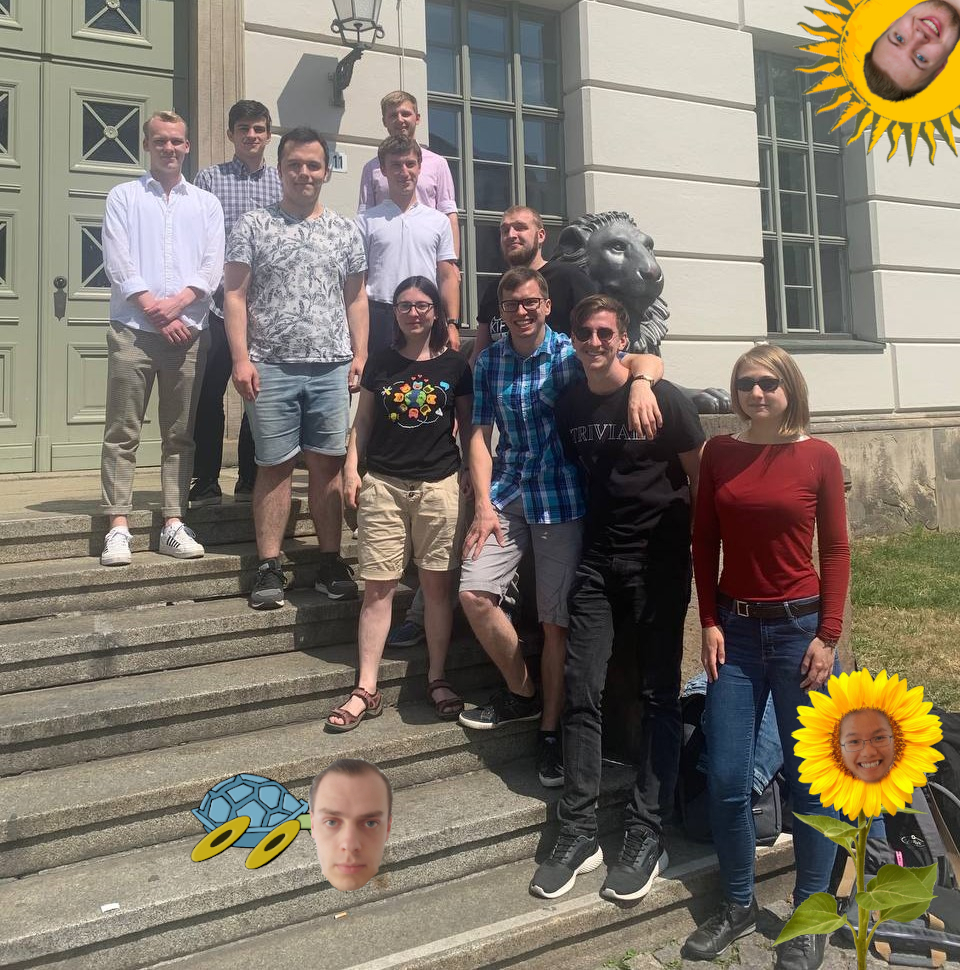
\includegraphics[width=1\linewidth]{fsr}
\end{center}%
FSR (v.l.n.r.): 
Stefan Beschke,
Aaron Gröbel, 
Jan Heinrich Reimer,  
Tuğçe Kuru, 
Anna Hemmann,
Marie Weise, 
Chris Juchum,  
Peter Böttcher.
Helfer (ohne Bild): Lenz Hank-Weise, Henrike Schweizer




\section{Studienordnung}
Hier geben wir dir einen Überblick
zur Studien- und Prüfungsordnung an der MLU.
\begin{center}
	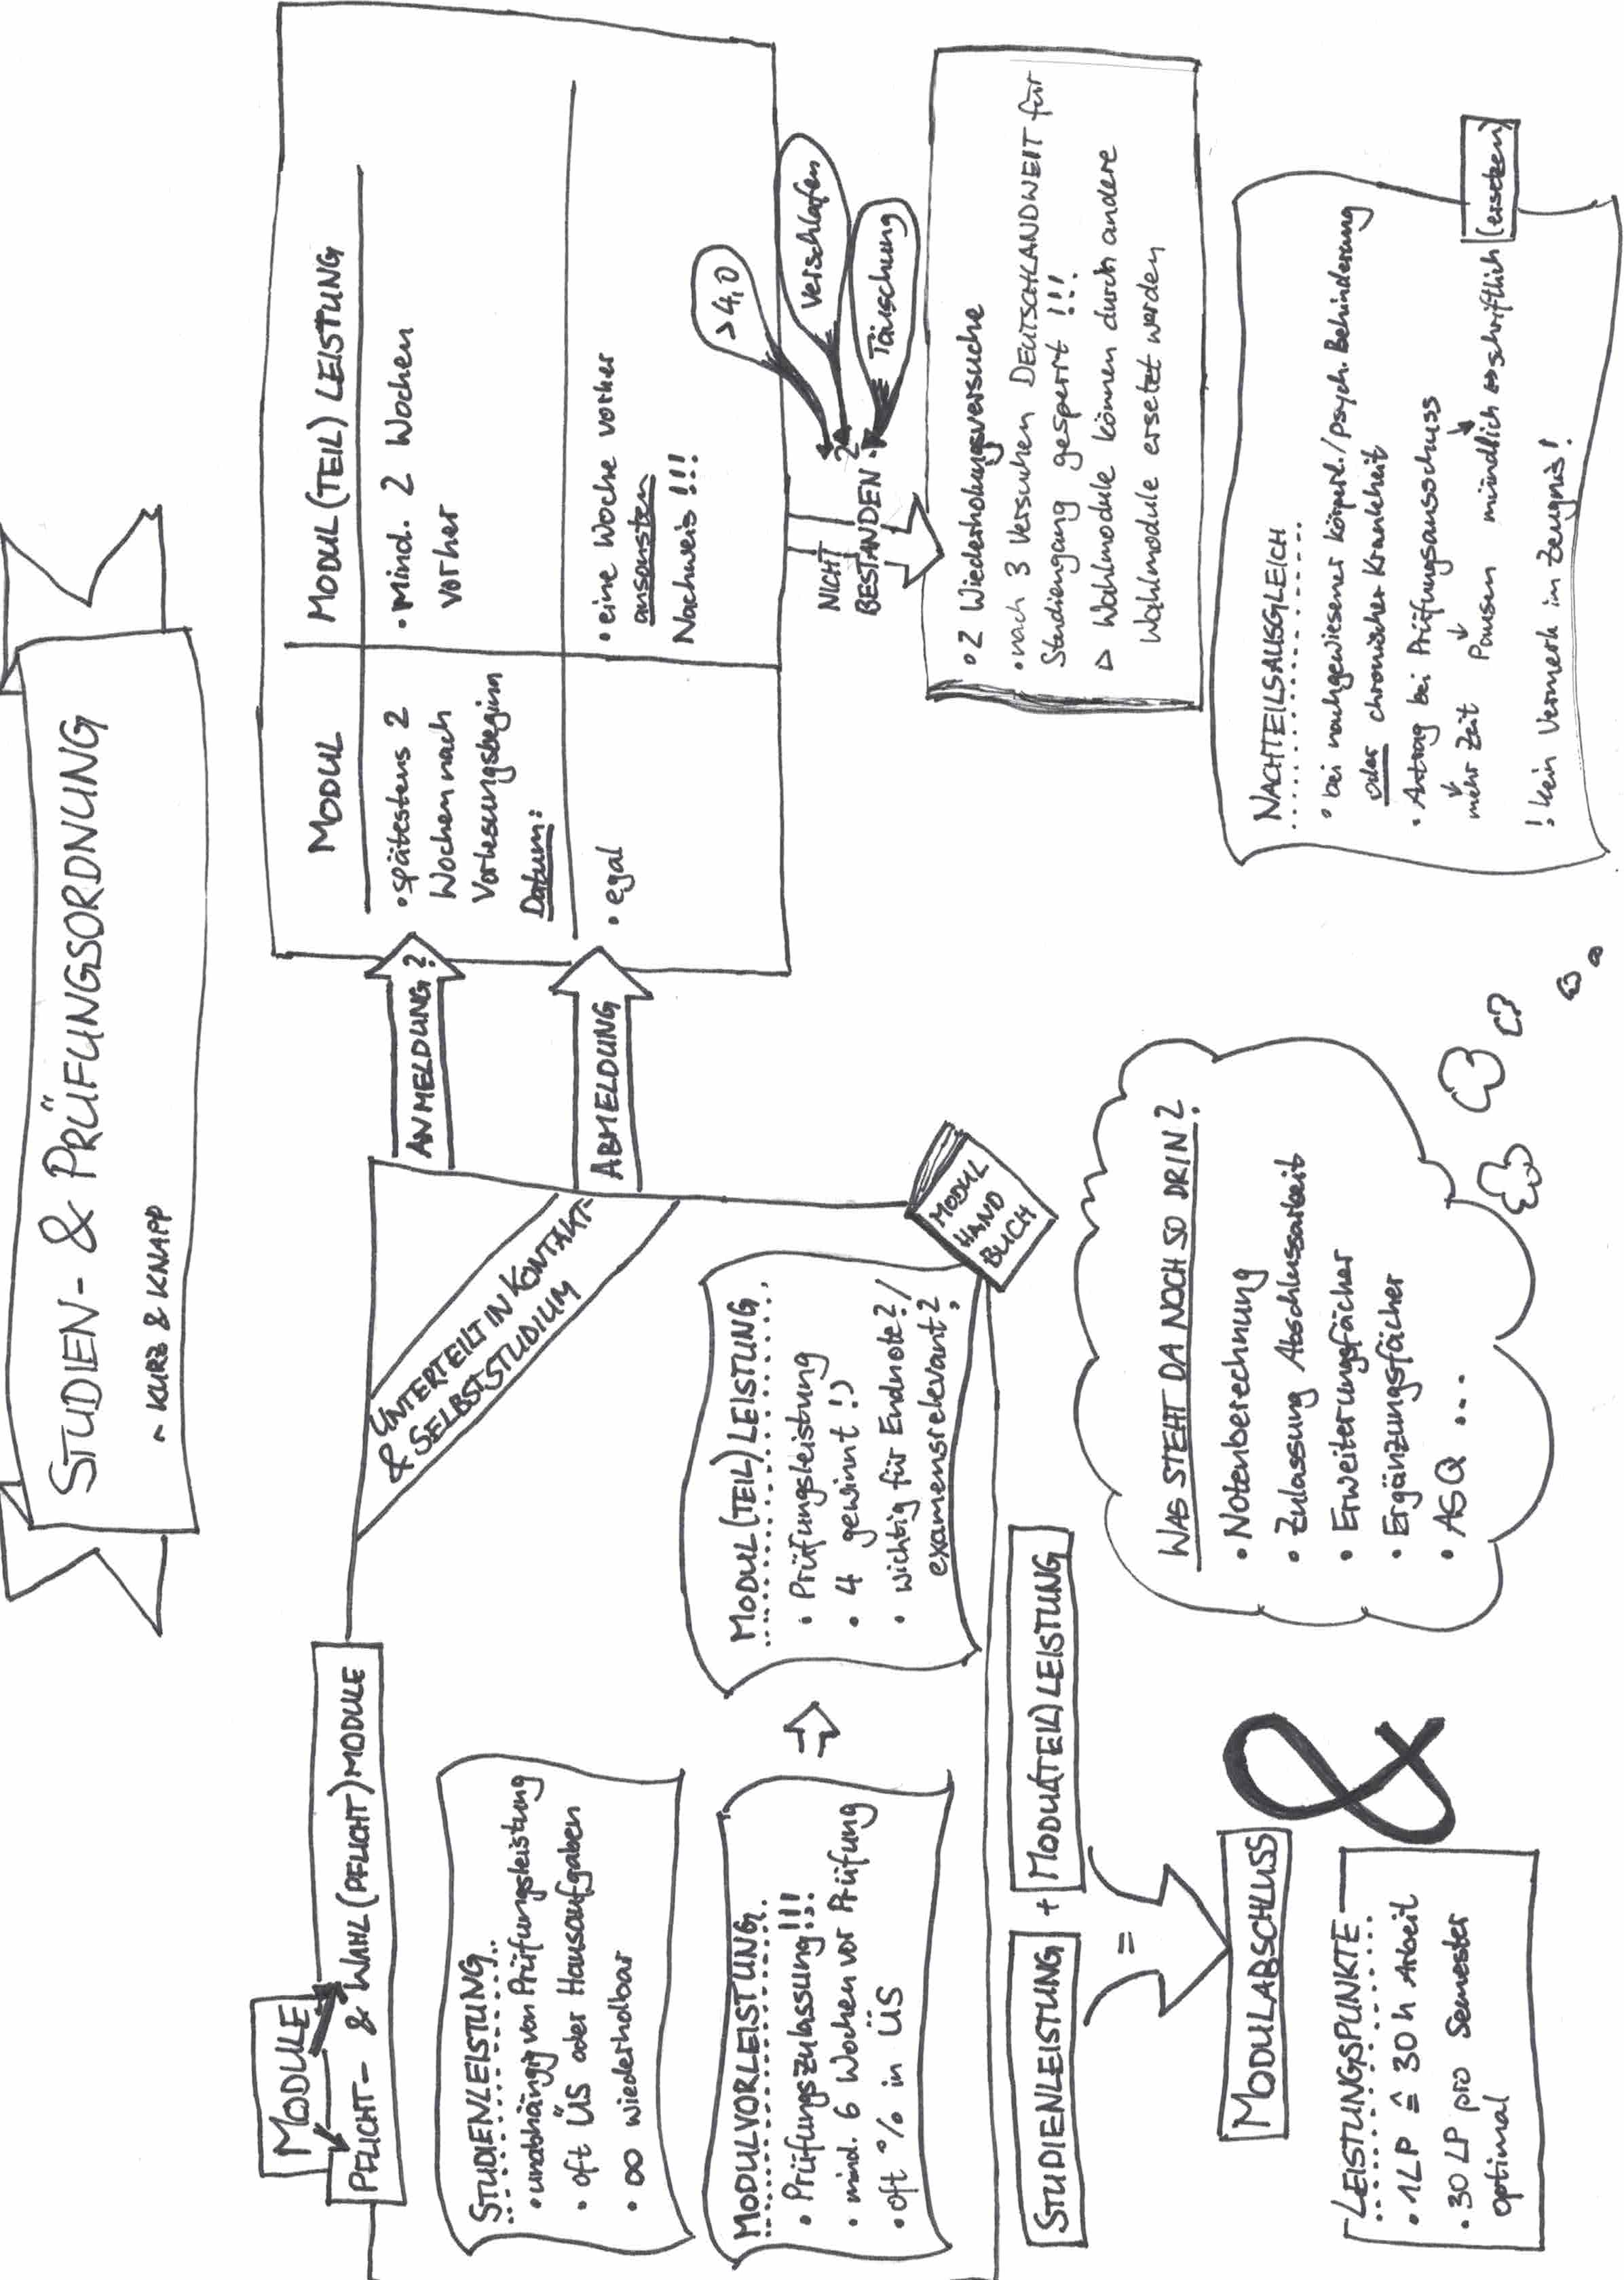
\includegraphics[width=0.89\textwidth]{studiordnung}
\end{center}

\section{Studiengänge}

Im folgenden findet ihr Auszüge aus den Modulhandbüchern und Empfehlungen aus den Regelstudienplänen, außerdem Ansprechpartner für Fragen und \textquote{Sonderwünsche}.
Fragen können immer auch an den FSR gerichtet werden.

\subsection{Studienberater}
\subsubsection{Mathematik/Wirtschaftsmathematik}
Dr.\ Hans-Georg Rackwitz \\
Theodor-Lieser-Str.~5, Raum~127 \\
Telefon: +49\,345\,55\,24608\\
E-Mail: \email{hans-georg.rackwitz@mathematik.uni-halle.de}\\

\subsubsection{Informatik/Bioinformatik}
Dr.\ Steffen Schüler \\
Von-Seckendorff-Platz~1, Raum~4.20 \\
Telefon: +49\,345\,55\,24735 \\
E-Mail: \email{steffen.schueler@informatik.uni-halle.de}

\subsubsection{Lehramt}
Zentrum für Lehrerbildung \\
Dr. Marie-Theres Müller \\
Dachritzstraße~12, Raum~205 \\
Telefon: +49\,345\,55\,21717 \\
E-Mail: \email{zlb@uni-halle.de}

\newpage

\section{Studiengangsübersichten}

\subsection{Informatik}
\label{studiengang_informatik}

\subsubsection{Regelstudienplan}
\begin{singlespace}
	\begin{small}
		\begin{longtabu} to \textwidth {X|r@{\hspace{0.75em}}r@{\hspace{0.75em}}r@{\hspace{0.75em}}r@{\hspace{0.75em}}r@{\hspace{0.75em}}r|r}
			\toprule
			\textbf{Modul}&\multicolumn{6}{l|}{\textbf{LP pro Semester}}&\textbf{LP}\\
			& 1. & 2. & 3. & 4. & 5. & 6. &\\
			\midrule
			\endfirsthead
			\midrule
			\textbf{Modul}&\multicolumn{6}{l|}{\textbf{LP pro Semester}}&\textbf{LP}\\
			& 1. & 2. & 3. & 4. & 5. & 6. &\\
			\midrule
			\endhead
			\midrule
			\endfoot
			\bottomrule
			\endlastfoot
			\multicolumn{8}{l}{\textbf{Informatik-Grundlagen}} \\
			Objektorientierte Programmierung & 5 & & & & & & 5 \\ 
			Einführung in die Rechnerarchitektur & 5 & & & & & & 5 \\ 
			Mathematische Grundlagen der Informatik \& Konzepte der Modellierung & 7 & 8 & & & & & 15 \\ 
			Einführung in Betriebssysteme & & 5 & & & & & 5 \\ 
			Einführung in die technische Informatik & & 5 & & & & & 5 \\ 
			Datenstrukturen \& effiziente Algorithmen~I & & 5 & & & & & 5 \\ 
			Konzepte der Programmierung & & & 5 & & & & 5 \\ 
			Automaten \& Berechenbarkeit & & & & 10 & & & 10 \\
			\midrule
			\multicolumn{8}{l}{\textbf{Mathematik}} \\
			Diskrete Strukturen, lineare Algebra \& Analysis (Mathe B) & 8 & 7 & & & & & 15 \\ 
			Einführung in Data Science & & & & 5 & & & 5 \\
			\midrule
			\multicolumn{8}{l}{\textbf{Informatik-Vertiefung}} \\
			Einführung in Datenbanken & & & 5 & & & & 5 \\ 
			Datenstrukturen \& effiziente Algorithmen~II & & & 5 & & & & 5 \\ 
			Softwaretechnik & & & 5 & & & & 5 \\ 
			Einführung in die Bildverarbeitung & & & 5 & & & & 5 \\
			Projektpraktikum & & & & 5 & 10 & & 15 \\ 
			Einführung in die Rechnernetze \& verteilte Systeme & & & & & 5 & & 5 \\  
			Gestaltung \& Durchführung von Fachvorträgen in der Informatik & & & & & 5 & & 5 \\
			\midrule
			\multicolumn{8}{l}{\textbf{Anwendungsfach, ASQ, Wahlpflicht}} \\
			Allgemeine Schlüsselqualifikationen (ASQ) & 5 & & & & & 5 & 10 \\
			Anwendungsfach & & & 5 & 5 & 5 & & 15 \\ 
			„Spezialisierung“\,/\,Wahlpflicht & & & & 5 & 5 & 10 & 20 \\ 
			\midrule
			\textbf{Bachelorarbeit} & & & & & & 15 & 15 \\
		\end{longtabu}
	\end{small}
\end{singlespace}

\subsection{Bioinformatik}
\label{studiengang_bioinformatik}

\subsubsection{Regelstudienplan}
\begin{singlespace}
	\begin{small}
		\begin{longtabu} to \textwidth {X|r@{\hspace{0.75em}}r@{\hspace{0.75em}}r@{\hspace{0.75em}}r@{\hspace{0.75em}}r@{\hspace{0.75em}}r|r}
			\toprule
			\textbf{Modul}&\multicolumn{6}{l|}{\textbf{LP pro Semester}}&\textbf{LP}\\
			& 1. & 2. & 3. & 4. & 5. & 6. &\\
			\midrule
			\endfirsthead
			\midrule
			\textbf{Modul}&\multicolumn{6}{l|}{\textbf{LP pro Semester}}&\textbf{LP}\\
			& 1. & 2. & 3. & 4. & 5. & 6. &\\
			\midrule
			\endhead
			\midrule
			\endfoot
			\bottomrule
			\endlastfoot
			\multicolumn{8}{l}{\textbf{Pflichtbereich Informatik}}\\ 
			Objektorientierte Programmierung & 5 & & & & & & 5 \\
			Grundlagen der Bioinformatik & 8 & 7 & & & & & 15 \\ 
			Datenstrukturen \& effiziente Algorithmen~I & & 5 & & & & & 5 \\ 
			Enführung in Datenbanken & & & 5 & & & & 5 \\ 
			Softwaretechnik & & & 5 & & & & 5 \\ 
			Algorithmen auf Sequenzen~I & & & & 5 & & & 5 \\ 
			Spezielle Probleme der Bioinformatik & & & & 5 & & & 5 \\ 
			Gestaltung \& Durchführung von Fachvorträgen in der Bioinformatik & & & & & 5 & & 5 \\
			Statistische Datenanalyse \& Maschinelles Lernen in der Bioinformatik~I & & & & & 5 & & 5 \\ 
			\midrule
			\multicolumn{8}{l}{\textbf{Pflichtbereich Mathematik}}\\ 
			Diskrete Strukturen, lineare Algebra \& Analysis (Mathe B) & 7 & 8 & & & & & 15 \\ 
			Einführung in Data Science & & & & 5 & & & 5 \\ 
			\midrule
			\multicolumn{8}{l}{\textbf{Pflichtbereich Biologie}}\\ 
			Biologie für Bioinformatiker~I (Zellbiologie, Botanik) & 8 & & & & & & 8 \\ 
			Biologie für Bioinformatiker~II (Mikrobiologie, Ökologie) & & 7 & & & & & 7 \\ 
			Biologie für Bioinformatiker~III (Genetik, Zoologie) & & & 10 & & & & 10 \\ 
			\midrule
			\multicolumn{8}{l}{\textbf{Pflichtbereich Biochemie}}\\
			Allgemeine Biochemie für Bioinformatiker & & & 10 & & & & 10 \\ 
			\midrule
			\multicolumn{8}{l}{\textbf{Pflichtbereich Chemie}}\\ 
			Organische Chemie im Nebenfach (OC-N) & 2 & 3 & & & & & 5 \\ 
			Physikalische Chemie für die Bioinformatik (PC-N~VI) & & & & 5 & & & 5 \\ 
			\midrule
			\multicolumn{8}{l}{\textbf{Pflichtbereich ASQ/Wahlpflicht}}        \\ 
			Allgemeine Schlüsselqualifikationen & & & & 5 & 5 & & 10 \\ 
			Wahlpflicht* & & & & 5 & 15 & 15 & 35 \\ 
			\midrule
			\textbf{Bachelorarbeit} & & & & & & 15 & 15 \\
		\end{longtabu}
	\end{small}
\end{singlespace}
Von den mit * markierten Wahlpflichtmodulen müssen jeweils mindestens 10~LP aus den Bereichen Informatik und Biowissenschaften erbracht werden.

\subsection{Informatik Lehramt}
\label{studiengang_infolehramt}

\subsubsection{Regelstudienplan}

\begin{singlespace}
	\begin{small}
		\begin{longtabu} to \textwidth {X|l|r}
			\toprule
			\textbf{Modul} & \textbf{Semester} & \textbf{LP} \\
			\midrule
			\endfirsthead
			\midrule
			\textbf{Modul} & \textbf{Semester} & \textbf{LP} \\
			\midrule
			\endhead
			\midrule
			\endfoot
			\bottomrule
			\endlastfoot
			\multicolumn{3}{l}{\textbf{Pflichtmodule Informatik}}\\
			Objektorientierte Programmierung & 1. & 5 \\
			Einführung in Rechnerarchitektur & 1. & 5 \\
			Mathematische Grundlagen der Informatik \& Konzepte der Modellierung & 1.\,--\,2. & 15 \\
			Datenstrukturen \& effiziente Algorithmen I & 2.\,/\,4. & 5 \\
			Technische Informatik, Betriebssysteme \& Rechnernetze (Lehramt) & 3. & 5 \\
			Konzepte der Programmierung & 3. & 5 \\
			Einführung in Datenbanken & 3.\,/\,5. & 5 \\
			Datenbank-Programmierung & 4.\,/\,6. & 5 \\
			Automaten \& Berechenbarkeit* & 4.\,/\,6. & 10 \\
			Softwaretechnik (Lehramt) & 5. & 5 \\
			Informatik \& Gesellschaft & \(\geq\) 5. & 5 \\
			\midrule
			\multicolumn{3}{l}{\textbf{Wahlmodule Informatik}}\\
			Wahlmodul I & \(\geq\) 5. & 5 \\
			Wahlmodul II* & \(\geq\) 5. & 5 \\
			\midrule
			\multicolumn{3}{l}{\textbf{Fachdidaktik Informatik}}\\
			Didaktik der Informatik AB & 3.\,/\,4. & 5 \\
			Didaktik der Informatik CDE & \(\geq\) 4. & 5 \\
			Didaktik der Informatik FG & \(\geq\) 5. & 5 \\
		\end{longtabu}
	\end{small}
\end{singlespace}
Die mit * gekennzeichnete Module sind nur von LAGs zu belegen.

\subsection{Mathematik}
\label{studiengang_mathematik}

\subsubsection{Regelstudienplan}

\begin{singlespace}
	\begin{small}
		\begin{longtabu} to \textwidth {X|r@{\hspace{0.75em}}r@{\hspace{0.75em}}r@{\hspace{0.75em}}r@{\hspace{0.75em}}r@{\hspace{0.75em}}r|r}
			\toprule
			\textbf{Modul}&\multicolumn{6}{l|}{\textbf{LP pro Semester}}&\textbf{LP}\\
			& 1. & 2. & 3. & 4. & 5. & 6. &\\
			\midrule
			\endfirsthead
			\midrule
			\textbf{Modul}&\multicolumn{6}{l|}{\textbf{LP pro Semester}}&\textbf{LP}\\
			& 1. & 2. & 3. & 4. & 5. & 6. &\\
			\midrule
			\endhead
			\midrule
			\endfoot
			\bottomrule
			\endlastfoot
			\multicolumn{3}{l}{\textbf{Pflichtbereich}}\\
			Objektorientierte Programmierung & 5 & & & & & & 5\\
			Analysis~I\,\&\,II & 9 & 9 & & & & & 18\\
			Lineare Algebra & 9 & 9 & & & & & 18\\
			Datenstrukturen \& effiziente Algorithmen~I & & 5 & & & & & 5\\
			Numerik~I\,\&\,II & & 9 & 9 & & & & 18\\
			Algebra & & & 9 & & & & 9\\
			Analysis~III & & & 9 & & & & 9\\
			Praktikum & & & & 6 & & & 6\\
			Maßtheorie & & & & 8 & & & 8\\
			Wahrscheinlichkeitstheorie \& Statistik & & & & 8 & & & 8\\
			Fachseminar & & & & & 5 & & 5\\
			Funktionalanalysis & & & & & 8 & & 8\\
			\midrule
			\multicolumn{3}{l}{\textbf{Wahlpflichtbereich}}\\
			Anwendungsfach & 5 & & & 5 & & 10 & 20\\
			Proseminar & & & 3 & & & & 3\\
			Allgemeine Schlüsselqualifikationen & & & & 5 & & 5 & 10\\
			Vertiefung Mathematik & & & & & 15 & & 15\\
			\midrule
			\textbf{Bachelorarbeit}& & & & & & 15 & 15\\
		\end{longtabu}
	\end{small}
\end{singlespace}

\subsection{Wirtschaftsmathematik}
\label{studiengang_wima}

\subsubsection{Regelstudienplan}

\begin{singlespace}
	\begin{small}
		\begin{longtabu} to \textwidth {X|r@{\hspace{0.75em}}r@{\hspace{0.75em}}r@{\hspace{0.75em}}r@{\hspace{0.75em}}r@{\hspace{0.75em}}r|r}
			\toprule
			\textbf{Modul}&\multicolumn{6}{l|}{\textbf{LP pro Semester}}&\textbf{LP}\\
			& 1. & 2. & 3. & 4. & 5. & 6. &\\
			\midrule
			\endfirsthead
			\midrule
			\textbf{Modul}&\multicolumn{6}{l|}{\textbf{LP pro Semester}}&\textbf{LP}\\
			& 1. & 2. & 3. & 4. & 5. & 6. &\\
			\midrule
			\endhead
			\midrule
			\endfoot
			\bottomrule
			\endlastfoot
			\multicolumn{8}{l}{\textbf{Pflichtbereich}}\\
			Objektorientierte Programmierung & 5 & & & & & & 5\\
			Analysis~I\,\&\,II & 9 & 9 & & & & & 18\\
			Lineare Algebra & 9 & 9 & & & & & 18\\
			Datenstrukturen \& effiziente Algorithmen~I & & 5 & & & & & 5\\
			Optimierung & & 10 & 10 & & & & 20\\
			Analysis~III & & & 9 & & & & 9\\
			Maßtheorie & & & & 8 & & & 8\\
			Numerik für Wirtschaftsmathematiker & & & & 8 & & & 8\\
			Praktikum & & & & 8 & & & 8\\
			Wahrscheinlichkeitstheorie \& Statistik & & & & 8 & & & 8\\
			Fachseminar & & & & & 5 & & 5\\
			Versicherungsmathematik \& Risikotheorie & & & & & 8 & & 8\\
			\midrule
			\multicolumn{3}{l}{\textbf{Wahlpflichtbereich}}\\
			ASQ & 5 & & & & & 5 & 10\\
			Vertiefung Informatik & & & 5 & & & & 5\\
			Vertiefung Wirtschaftswissenschaften & & & 5 & & 10 & 10 & 25\\
			Vertiefung Mathematik & & & & & 5 & & 5\\
			\midrule
			\textbf{Bachelorarbeit}& & & & & & 15 & 15\\
		\end{longtabu}
	\end{small}
\end{singlespace}

\subsection{Mathematik Lehramt}
\label{studiengang_lehramt}

\subsubsection{Regelstudienplan Gymnasium}
\label{studiengang_lag}

Bei den mit * gekennzeichneten Teilgebieten muss jeweils nur ein Modul besucht werden.

\begin{singlespace}
	\begin{small}
		\begin{longtabu} to \textwidth {X|l|r}
			\toprule
			\textbf{Modul} & \textbf{Semester} & \textbf{LP} \\
			\midrule
			\endfirsthead
			\midrule
			\textbf{Modul} & \textbf{Semester} & \textbf{LP} \\
			\midrule
			\endhead
			\midrule
			\endfoot
			\bottomrule
			\endlastfoot
			Analysis~I \& II & 1.\,--\,2. & 15\\
			Lineare Algebra & 1.\,--\,2. & 15\\
			Wahrscheinlichkeitstheorie \& Statistik & 4.\,/\,6. & 6\\
			Proseminar & \(\geq\) 3. & 5\\
			Grundlagen der numerischen Mathematik & \(\geq\) 3. & 5\\
			Algebra & \(\geq\) 3. & 7\\
			Fachseminar & \(\geq\) 5. & 5\\
			Vertiefungsmodul (nur wenn Erstfach)& \(\geq\) 3.& 5\\
			Mathematikdidaktik~I & 3.\,--\,4. & 5\\
			Mathematikdidaktik~II & 4.\,--\,5. & 5\\
			Mathematikdidaktik~III & 6.\,--\,7. & 5\\
			\midrule
			\multicolumn{3}{l}{\textbf{Wahlpflichtbereich Geometrie*}}\\
			Geometrie & 5.\,/\,7. & 7\\
			Differentialgeometrie & 5.\,/\,7. & 7\\
			\midrule
			\multicolumn{3}{l}{\textbf{Wahlpflichtbereich Grundlagen*}}\\
			Geschichte der Mathematik & \(\geq\) 4.& 5\\
			Grundlagen der Mathematik & \(\geq\) 4.& 5\\
			\midrule
			\multicolumn{3}{l}{\textbf{Wahlpflichtbereich Analysis/Numerik*}}\\
			Funktionentheorie & \(\geq\) 5.& 5\\
			Gewöhnliche Differentialgleichungen& \(\geq\) 5.& 5\\
			Theorie \& Numerik gewöhnlicher Dgl.& \(\geq\) 5.& 5\\
		\end{longtabu}
	\end{small}
\end{singlespace}

\subsubsection{Regelstudienplan Sekundarschule}
\label{studiengang_las}

Bei dem mit * gekennzeichneten Teilgebiet müssen zwei Module besucht werden.

\begin{singlespace}
	\begin{small}
		\begin{longtabu} to \textwidth {X|l|r}
			\toprule
			\textbf{Modul} & \textbf{Semester} & \textbf{LP} \\
			\midrule
			\endfirsthead
			\midrule
			\textbf{Modul} & \textbf{Semester} & \textbf{LP} \\
			\midrule
			\endhead
			\midrule
			\endfoot
			\bottomrule
			\endlastfoot
			Lineare Algebra & 1.\,--\,2. & 15\\
			Elemente der Mathematik & 1.\,--\,2. & 5\\
			Analysis~I & 3.& 10\\
			Elemente der Kombinatorik \& Stochastik & 3.\,/\,5. & 5\\
			Elemente der Geometrie & 3.\,/\,5. & 5\\
			Proseminar & 3.\,--\,6. & 5 \\
			Algebra & 3.\,/\,5. & 5\\
			Vertiefungsmodul (nur wenn Erstfach)& 4.\,--\,8. & 5\\
			Mathematikdidaktik~I & 3.\,--\,4. & 5\\
			Mathematikdidaktik~II & 4.\,--\,5. & 5\\
			Mathematikdidaktik~III & 6.\,--\,7. & 5\\
			\midrule
			\multicolumn{3}{l}{\textbf{Wahlpflichtbereich Mathematik*}}\\
			Analysis~II & 4.\,/\,6.  & 5\\
			Geschichte der Mathematik & 4.\,/\,6.  & 5\\
			Grundlagen der numerischen Mathematik & 5.\,/\,7.  & 5\\
			Funktionentheorie & 5.\,/\,7. & 5\\
			Geometrie & 5.\,/\,7. & 5\\
			Diskrete Mathematik & 5.\,/\,7. & 5\\
		\end{longtabu}
	\end{small}
\end{singlespace}


\section{Lexikon}

\begin{encyclopedia}
    \definition{akademisches Viertel}{
        siehe cum tempore.
    }
    \definition{BAFöG}{
        Bundesausbildungsförderungsgesetz.
        Regelt die finanzielle Unterstützung von Studierenden
        durch den Staat in Form von Stipendium und Darlehen.
        siehe auch BAFöG-Amt.
    }
    \definition{cum tempore}{
        Das \textquote{akademische Viertel}, eine Viertelstunde,
        wird der angegebenen Zeit hinzugerechnet, z.B.: 14:00~c.t. = 14:15~Uhr.
    }
    \definition{c.t.}{
        siehe cum tempore.
    }
    \definition{sine tempore}{
        Die angegebene Zeit ist wörtlich zu verstehen, z.B.: 14:00~s.t. = 14:00~Uhr.
    }
    \definition{s.t.}{
        siehe sine tempore.
    }
    \definition{DekanIn}{
        Oberhaupt einer Fakultät,
        SprecherIn des Fakultätsrates.
    }
    \definition{dies academicus}{
        Feiertag an der Uni,
        an dem keine Vorlesungen oder Übungen stattfinden.
        Findet 1--2 mal im Semester zu besonderen Veranstaltungen statt.
    }
    \definition{Fakultät}{
        Gruppierung von Instituten.
        Die MLU besteht aus 10~Fakultäten.
        Das Institut für Mathematik ist in der
        Naturwissenschaftlichen Fakultät~II (NatFak~II),
        das Institut für Informatik in der
        Naturwissenschaftlichen Fakultät~III (NatFak~III).
    }
    \definition{HiWi}{
        Hilfswissenschaftler bzw. Wissenschaftliche Hilfskraft.
        HiWis sind in der Regel selbst Studenten,
        meist höheren Semesters.
    }
    \definition{Hochschulgesetz}{
        Landeshochschulgesetz (HSG~LSA).
        Regelt Strukturen der Hochschulen in Sachsen-Anhalt,
        definiert Inhalt des Studiums,
        legt fest, wer studieren darf etc.
    }
    \definition{(IT)\textsuperscript{2}}{
        Industrietag~Informationstechnik.
        Fachtagung des UZI.
        Findet jedes Semester statt.
    }
    \definition{ITZ}{
        IT-Servicezentrum.
        \url{https://itz.uni-halle.de/}
    }
    \definition{KanzlerIn}{
        VerwaltungschefIn der Uni.
    }
    \definition{KommilitonIn}{
        Mitstudierende, Studiengenosse.
    }
    \definition{Mensa}{
        Speisehaus für Studierende mit vergünstigtem Essen.
    }
    \definition{MLU}{
        Kürzel für die Martin-Luther-Universität~Halle-Wittenberg
    }
    \definition{RektorIn}{
        Akademisches Oberhaupt, repräsentiert die Universität.
    }
    \definition{Senat}{
        Oberstes beschlussfassendes Organ der gesamten Universität.
        Zuständig für die meisten Entscheidungen zu Forschung und Studium.
    }
    \definition{SoSe}{
        Sommersemester.
        Vom 01.04. bis zum 30.09.
    }
    \definition{SS}{
        siehe SoSe.
    }
    \definition{StuRa}{
        Studierendenrat.
        Oberstes Organ der studentischen Selbstverwaltung.
        \url{https://stura.uni-halle.de/}
    }
    \definition{SWS}{
        Semesterwochenstunden.
        Stunden je Woche im Semester, z.B.: Modul mit 4+2~SWS bedeutet jede Woche
        4~Stunden Vorlesung und 2~Stunden Übung.
    }
    \definition{ULB}{
        Universitäts- und Landesbibliothek.
        Katalog unter \url{https://lhhal.gbv.de/}.
        \url{https://bibliothek.uni-halle.de/}
    }
    \definition{Bib}{
        siehe ULB.
    }
    \definition{Bibliothek}{
        siehe ULB.
    }
    \definition{USZ}{
        Universitätssportzentrum.
        Anmeldung für Kurse online: \url{https://usz.uni-halle.de/}.
        Unbedingt rechtzeitig am Mittwoch der ersten Vorlesungswoche anmelden.
    }
    \definition{UZI}{
        Universitätszentrum für Informatik.
        \url{https://uzi.uni-halle.de/}
    }
    \definition{WiSe}{
        siehe WS.
    }
    \definition{WS}{
        Wintersemester.
        Vom 01.10. bis zum 31.03.
    }
    \definition{VSP}{
        Von-Seckendorff-Platz.
        Informatikseite am Heidecampus.
    }
    \definition{VDP}{
        Von-Danckelmann-Platz.
        Physikseite am Heidecampus.
    }
    \definition{TLS}{
        Theodor-Lieser-Straße.
        Straße an der Heidemensa.
    }
    \definition{Cantor-Haus}{
        Heimat des Instituts für Mathematik.
    }
    \definition{AudiMax}{
        Größter Hörsaal, am Hauptcampus.
    }
    \definition{Mel}{
        Melanchtonianum, Hörsaalgebäude am Hauptcampus.
    }
    \definition{Hauptcampus}{
        Zentraler Campus am Universitätsplatz.
    }
    \definition{Kleine Ulli}{
        Kleine Ulrichstraße.
        Kneipenstraße in der Innenstadt.
    }
    \definition{LP}{
        Leistungspunkte.
        Bekommt man für jedes Modul.
        Zum Erreichen des Abschlusses notwendig.
    }
    \definition{CP}{
        Credit Points, siehe LP.
    }
    \definition{ZLB}{
        Zentrum für Lehrerbildung.
        In der Nähe des Hauptcampus.
        Koordination und Beratung für das Lehramtsstudium.
    }
    \definition{ASQ}{
        Allgemeine Schlüsselqualifikationen.
        Fachfremde Wahlpflichtmodule.
        Soll \textquote{Fachidioten} vorbeugen.
    }
    \definition{FSR}{
        Fachschaftsrat
        \begin{itemize}[noitemsep]
            \item Studierendenvertretung / Interessenvertretung
            \item für Fachbereiche Mathematik und Informatik
            \item 13~Mitglieder
            \item jährlich gewählt im Mai
            \item zahlreiche Veranstaltungen, u.a. Spieleabende, Weihnachtsfeier, NatFusion, Sommerfest
            \item freier Eintritt, günstige Verpflegung bei allen Veranstaltungen.
            \item Bindeglied zu ProfessorInnen und MitarbeiterInnen
            \item finanziert Anschaffungen für die Studierenden
            \item AnsprechpartnerInnen für Fragen und Probleme
            \item finanziert sich aus einem Teil des Semesterbeitrags (\EUR{11,95}~pro Semester)
            \item öffentliche Sitzung im Semester vsl. donnerstags 18 Uhr
            \item alle dürfen mitmachen -- lass dich wählen
        \end{itemize}
        \url{https://fachschaft.mathinf.uni-halle.de}\\
        \email{fachschaft@mathinf.uni-halle.de} \\
        Instagram: fsr.matheinfo.halle \\
        Von-Seckendorff-Platz 1, Raum 0.31
    }
    \definition{Fachschaft}{
        siehe FSR.
    }
    \definition{Spieleabend}{
        Spiel, Spaß und Bier mit Karaoke.
        Veranstaltung des FSR.
    }
    \definition{Weihnachtsfeier}{
        Kekse, Glühwein und Schrottwichteln in Weihnachtsatmosphäre.
        Veranstaltung des FSR.
    }
    \definition{NatFusion}{
        Open-Air-Party im Frühjahr mit der Physik, Chemie, Biochemie.
        Veranstaltung des FSR.
    } 
    \definition{Sommerfest}{
        Outdoor-Spieleabend mit Festplatten-Zielwurf.
        Veranstaltung des FSR.
    }
    \definition{Tutorium}{
        Zusätzliche Übungsmöglichkeit zum Vorlesungsinhalt.
        Wird oft von älteren Studierenden geleitet.
    }
    \definition{Übung}{
        Besprechung des Vorlesungsinhalts,
        Bearbeiten von Übungsaufgaben,
        Besprechen der Übungsserien.
        Manchmal Anwesenheitspflicht.
    }
    \definition{Übungsserie}{
        Verpflichtende Vor- oder Teilleistung.
        Meist müssen ca. 50\% der Punkte erreicht werden.
        Häufig kann in Gruppen gearbeitet werden.
    }
    \definition{Hausaufgabe}{
        siehe Übungsserie.
    }
    \definition{Vorlesung}{
        Vortrag der Dozentin oder des Dozenten über das Modulthema.
    }
    \definition{Club}{
        siehe Nachtleben.
    }
    \definition{Bar}{
        siehe Nachtleben.
    }
    \definition{Restaurant}{
        Viele Restaurants in der Kleinen Ulli und Sternstraße.
    }
    \definition{Sternstraße}{
        Straße mit vielen Restaurants.
    }
    \definition{Nachtleben}{
        u.a. Turm, Palette, Druschba, 
        Schorre, Charles Bronson, Flo-Po,
        Enchi, Bauernclub, Objekt~5.
        Weitere: \url{https://kulturfalter.de/}
    }
    \definition{Palette}{
        Tanzbar.
    }
    \definition{Druschba}{
        Club.
    }
    \definition{Schorre}{
        Club.
    }
    \definition{Objekt~5}{
        Bar.
    }
    \definition{Charles Bronson}{
        Club.
    }
    \definition{Turm}{
        Club in der Moritzburg.
    }
    \definition{Flo-Po}{
        Flower-Power.
        Musikkneipe mit Karaoke.
    }
    \definition{Enchi}{
        Enchilada.
        Mexikanische Cocktailbar am Hauptcampus.
        Montags Cocktailwürfeln.
    }
    \definition{Bauernclub}{
        Studentenclub.
    }
    \definition{hastuzeit}{
        Studierendenzeitschrift über Studierendenalltag,
        Hochschulpolitik und Erfahrungen mit Auslandssemestern.
        Vom StuRa herausgegeben.
        \url{https://hastuzeit.de/}
    }
    \definition{Fakultätsrat}{
        Vertretung der ProfessorInnen, 
        Studierenden und MitarbeiterInnen einer Fakultät.
    }
    \definition{MDV}{
        Mitteldeutscher Verkehrsbund.
        Regionalverkehr in der Region Leipzig/Halle.
        Gültigkeitsbereich des Semestertickets
        (nicht gültig für MDV-Norderweiterung!)
    }
    \definition{Semesterticket}{
        Verkehrsticket im Studierendenausweis,
        gültig im MDV-Gebiet
        (ausgenommen MDV-Norderweiterung!)
    }
    \definition{Studierendenausweis}{
        Universeller Ausweis fürs Studium.
        Immer dabei haben, jedes Semester rechtzeitig validieren!
        \begin{itemize}[noitemsep]
            \item Mensa
            \item Drucken/Kopieren
            \item Bibliothek
            \item Semesterticket
            \item Identitätsnachweis für Prüfungen und Wahlen
            \item Schlüsselkarte
            \item Ermäßigungskarte im öffentlichen Leben
        \end{itemize}
        Validierungsstellen im Löwengebäude,
        der Heidemensa, der Weinbergmensa,
        und Haus 31 in den Franckeschen Stiftungen.
    }
    \definition{Studentenwerk}{
        Sozialer Service für Studierende
        \begin{itemize}[noitemsep]
            \item BAFöG
            \item Mensa
            \item Wohnen
            \item Beratung
            \item Kinderbetreuung
            \item Kultur
        \end{itemize}
        \url{https://studentenwerk-halle.de/}
    }
    \definition{Studieren mit Kind}{
        Kitas, Vergünstigungen etc. vom Studentenwerk. Im GCH gibt es einen Raum, der extra für Studis und Angestellte mit Kindern eingerichtet ist. 
        \url{https://uni-halle.de/familiengerecht}
    }
    \definition{Stipendium}{
        Förderung aus Stiftungen und Wirtschaft 
        zur finanziellen Unterstützung im Studium.
        Übersicht auf \url{https://stipendienlotse.de/}.
    }
    \definition{Mathe-Treff}{
        Treffpunkt für ratlose Studis,
        Unterstützung bei allen Mathe-Fragen.
        Täglich geöffnet: R\,1.30 im Cantor-Haus.
        \url{https://studieninfo.mathematik.uni-halle.de/mathe-treff/}
    }
    \definition{Info-Treff}{
        Treffpunkt für ratlose Studis,
        Unterstützung bei allen Info-Fragen.
        Di. bis Fr. geöffnet: R\,5.08 im VSP.
    }
    \definition{Mentoring}{
        Mentoringprogramm für Bioinformatiker.
        \url{https://studieninfo.informatik.uni-halle.de/unser-institut/mentoring/}
    }
    \definition{LaTeX}{
        Textsatzprogramm.
        Gut geeignet für mathematische und wissenschaftliche Texte.
        Von Professoren bevorzugt; besser als Word.
        LaTeX-Kurs des FSR oder LaTeX-ASQ besuchen.
        LaTeX-Vorlage unter \url{https://fachschaft.mathinf.uni-halle.de/informationen/latex}.
    }
    \definition{Pool}{
        siehe Computerpool.
    }
    \definition{Computerpool}{
        In der 3. Etage im VSP.
        Kostenlose Druckseiten.
        \url{https://informatik.uni-halle.de/studium/pools/}
    }
    \definition{WLAN}{
        Uniweites kostenloses WLAN über das DFN.
        Einrichtung unter \url{https://wlan.itz.uni-halle.de/}.
        Siehe auch eduroam.
    }
    \definition{eduroam}{
        Weltweites kostenloses WLAN.
        Einrichtung unter \url{https://cat.eduroam.org/}.
    }
    \definition{DFN}{
        Deutsches Forschungsnetzwerk.
        Universitäres (ziemlich schnelles) Breitbandnetz.
        \url{https://dfn.de/}
    }
    \definition{Campus}{
        Ort des universitären Geschehens.
    }
    \definition{Tulpe}{
        Burse zur Tulpe. Mensa am Hauptcampus.
    }
    \definition{Löwengebäude}{
        Zentrales, representatives Gebäude am Hauptcampus.
    }
    \definition{Imma-Amt}{
        Immatrikulationsamt im Löwengebäude.
    }
    \definition{Prüfungsamt}{
        Anlaufstelle für Probleme bei der Modul-/Prüfungsanmeldung im Löwenportal. \\
        Info\,/\,NatFak~III: \url{https://natfak3.uni-halle.de/pruefungsamt\_natfak\_3/} \\
        Mathe\,/\,NatFak~II: \url{http://natfak2.uni-halle.de/studium/}
    }
    \definition{Löwenportal}{
        Online-Plattform für Uni-Bürokratie.
        Modul-, Prüfungsanmeldung, Bescheinigungen, Rückmeldung.
        \url{https://loewenportal.uni-halle.de/}
    }
    \definition{BAFöG-Amt}{
        Anlaufstelle für Probleme mit BAföG, in der Weinbergmensa. 
        \sloppy\url{https://studentenwerk-halle.de/bafoeg-studienfinanzierung/bafoeg/allgemeine-infos-zum-bafoeg/}
    }
    \definition{Ersti}{
        Erstsemester, das bist zum Beispiel du.
    }
    \definition{Uni-Sport}{
        siehe USZ.
    }
    \definition{Studienleistung}{
        Teilleistung zum Bestehen des Moduls.
    }
    \definition{Modulleistung}{
        Hauptleistung zum Bestehen des Moduls.
    }
    \definition{Modulvorleistung}{
        Vorleistung zur Anmeldung der Modulprüfung.
    }
    \definition{Modul}{
        Themenbezogene Vorlesungsreihe.
        Unterteilung des Gesamtstudiums.
        Beim erfolgreichen Abschluss bekommt man LP.
    }
    \definition{Anwendungsfach}{
        Für Informatik, fachfremde Module 
        zur Anwendung der informatischen Kenntnisse.
    }
    \definition{Spezialisierung}{
        Wahlpflichtmodule in der Informatik.
    }
    \definition{Selbststudium}{
        Zeit außerhalb des Stundenplans 
        zur Vor- und Nacharbeit der Vorlesung.
    }
    \definition{Heidecampus}{
        Campus der Naturwissenschaften, insb. Mathe/Info.
    }
    \definition{Weinbergcampus}{
        Campus der Chemie/Biologie.
    }
    \definition{Theater}{
        u.a. Opernhaus, Neues Theater, Thalia-Theater, Puppentheater. 
        \url{https://buehnen-halle.de/}
    }
    \definition{Kino}{
        u.a. Unikino, CinemaxX, thelight Cinema, Puschkino, Lux-Kino, Zazie.
    }
    \definition{Stud.IP}{
        Vorlesungs- und Austauschportal.
        Termine, Skripte, Lernübungen, Dateien, Kontakte.
        \url{https://studip.uni-halle.de/}
    }
    \definition{E-Mail}{
        Offizielle Uni-Mails über Studmail.
        \url{https://studmail.uni-halle.de/}.
        Regelmäßig lesen und/oder weiterleiten!
    }
    \definition{Mail}{
        siehe E-Mail.
    }
    \definition{SSC}{
        Studierenden-Service-Center.
        Immatrikulationsamt und allgemeine Studienberatung.
        \url{https://uni-halle.de/ssc/}.
    }
    \definition{International Office}{
        Organisation für Auslandssemester.
        \url{https://www.international.uni-halle.de/}
    }
    \definition{MLUconf}{
        Videokonferenz-Dienst der MLU, für datensichere Online-Vorlesungen und -Übungen,
        basierend auf Big Blue Button.
        Kann von Studierenden auch privat genutzt werden.
        \url{https://mluconf.uni-halle.de/}
    }
    \definition{MLUchat}{
        Chat-Dienst der MLU, für datensichere Absprachen mit Kommilitonen und Profs.
        \url{https://chat.uni-halle.de/}
    }
    \definition{Rocket.Chat}{
        siehe MLUchat.
    }
    \definition{Webex}{
        Lizensierter Videokonferenz-Dienst von Cisco, für Online-Vorlesungen und -Übungen.
        \url{https://uni-halle.webex.com/}
    }
    \definition{BBB}{
        siehe Big Blue Button.
    }
    \definition{Big Blue Button}{
        Open-Source Videokonferenz-Dienst, v.a. genutzt von MLUconf.
    }
    \definition{Opencast}{
        Open-Source Videostreaming-Dienst, v.a. für Vorlesungsaufzeichnungen im Stud.IP.
    }
    \definition{ILIAS}{
        Plattform für Online-Prüfungen,~-Kurse und Selbsttests zum Lernen, verknüpft im Stud.IP.
    }
    \definition{Übungsportal}{
        Plattform zum Hochladen der wöchentlichen Übungsserien, verknüpft im Stud.IP.
    }
    \definition{YAPEX}{
        Programmierumgebung für OOP-Übungen, verknüpft im Übungsportal.
    }
    \definition{LLZ}{
        Zentrum für multi­mediales Lehren und Lernen.
        \url{https://llz.uni-halle.de/}
    }
    \definition{GCH}{
        Georg-Cantor-Haus an der Theodor-Lieser-Straße. Institut für Mathematik.
    }
    
    \definition{Erasmus}{
        Förderprogramm für Studierende, die ein Auslandssemester planen.
    }
\end{encyclopedia}


% Leere Seiten erzeugen, damit der farbige Einband nicht bedruckt wird.
\whiledo{\intcalcMod{\value{page} + 2}{4} > 0}{
    \newpage\thispagestyle{empty}~
    \ifthenelse{\intcalcMod{\value{page} + 2}{4} = 0}{\pagecolor{coverbackground}}{}
}


\end{document}
